\section{Vorbereitungsphase}
14.02. - 27.02.
Die Arbeiten am Projekt begannen mit der Vorbereitungsphase. Das Zeil dieser war es, wichtige Abklärungen zu machen und Entscheidungen zu treffen damit im ersten Sprint mir der eigentlichen Entwicklung begonnen werden konnte.
Dies beinhaltete zum einen eine Befragung potenzieller Benutzer der zu entwickelnden Applikation sowie die Evaluation eines geeigneten Technologiestacks.
Mit einer Dauer von zwei Wochen war die Vorbereitungsphase gleich lang, wie ein Sprint. Bei ihr handelt es sich jedoch nicht um einen richtigen Sprint, da noch kein Backlog mit User Stories vorhanden war.
Der Backlog für die Sprints wurde währen dieser Phase basierend auf den Erkenntnissen der zuvor genannten Punkte erstellt.
In den folgenden Abschnitten wird die Umsetzung der Vorbereitungsphase detailliert beschrieben.

\subsection{Nutzerbefragung}
Wie im Kapitel TODO erklärt, ist der Auftrag dieses Projekts, eine bestehende Anwendung, DMT2, durch einen Neuentwicklung zu ersetzen.

Am Standort Cham der Landis+Gyr gibt es zwei Entwicklerteams, welche den DMT2 regelmässig verwenden.
% TODO öppis zu dene Teams schriibe, Hinweis, der Autor dieser Arbeit ist ebenfalls teils eines dieser Teams
Für dieses Projekt wurden die Mitglieder dieser beiden Teams als Nutzer definiert und in dieser Arbeit so bezeichnet.  % chamer das besser formuliere?
Zu Beginn der Vorbereitungsphase wurden alle Nutzer zu einem Meeting eingeladen.
In diesem Meeting wurden erörtert, welche Dinge bei der bestehende Anwendung bereits gut funktionieren und welche als störend wahrgenommen werden.
Ebenfalls wurde von den Nutzern Ideen \& Wünsche für die Neuentwicklung abgeholt.

Für das sammeln der Antworten wurde während des Meetings retrotool.io TODO eingesetzt.
Die Abbildungen \ref{fig:WhatWorksWell}, \ref{fig:WhatBothersYou} und \ref{fig:IdeasAndWishes} sind Screenshots daraus.

% todo In einem anderen Kapitel die Resultate der Umfrage aufarbeiten und hier referenzieren
% https://retrotool.io/8mWyxCzpbIfQPydp2FPf4


\begin{figure}[H]
   \centering
   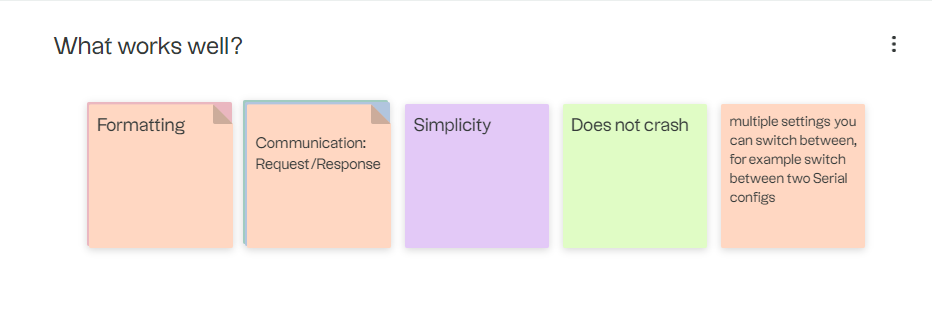
\includegraphics[width=1.0\textwidth]{gfx/S1_RetroBoard_WhatWorksWell.png}
   \caption{
       Antworten der Nutzer zur Frage "Was funktioniert bereits gut?"
   }
   \label{fig:WhatWorksWell}
\end{figure}

\begin{figure}[H]
   \centering
   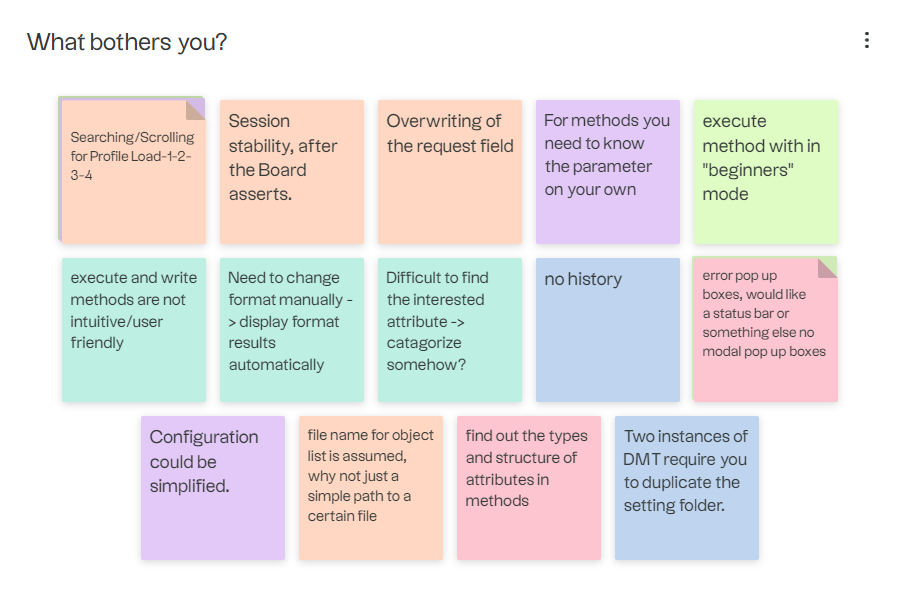
\includegraphics[width=1.0\textwidth]{gfx/S1_RetroBoard_WhatBothersYou.png}
   \caption{
       Antworten der Nutzer zur Frage "Was stört dich?"
   }
   \label{fig:WhatBothersYou}
\end{figure}

\begin{figure}[H]
   \centering
   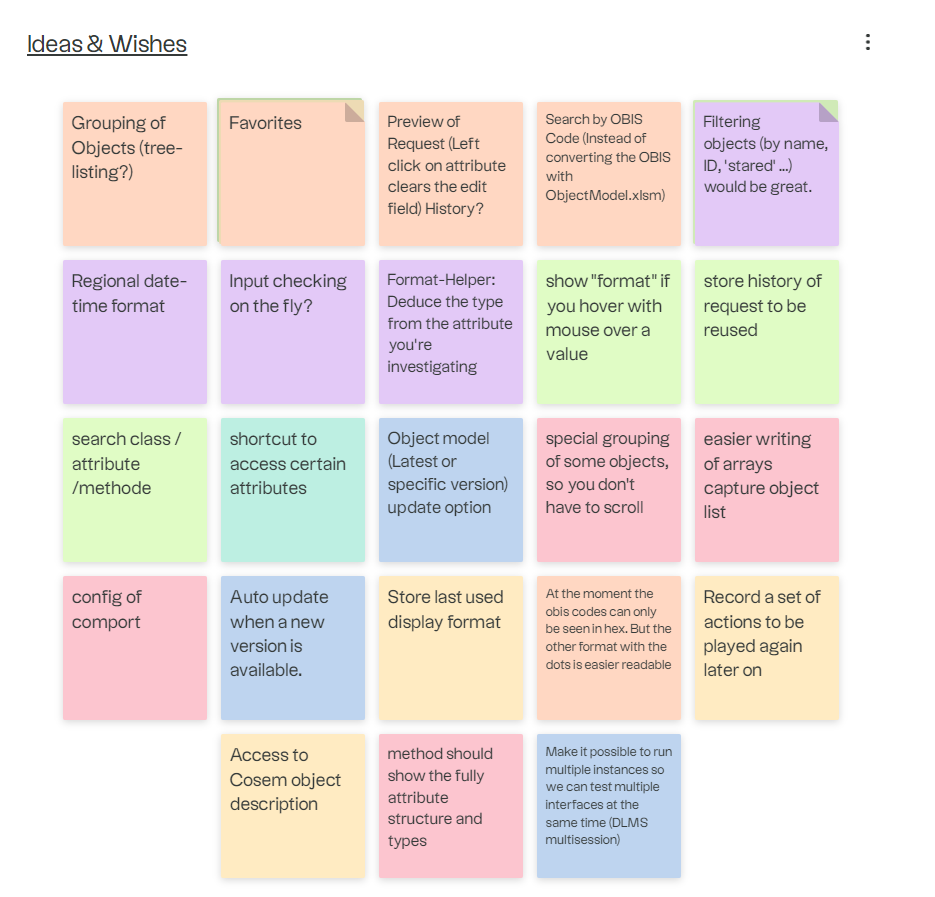
\includegraphics[width=1.0\textwidth]{gfx/S1_RetroBoard_IdeasAndWishes.png}
   \caption{
       Ideen und Wünsche der Nutzer an die neue Anwendung.
   }
   \label{fig:IdeasAndWishes}
\end{figure}

Um die Prioritäten der gesammelten Ideen \& Wünsche herauszufinden, wurde anschliessend an das Meeting eine Umfrage durchgeführt.
Ein Teil dieser Umfrage war es, dass die Nutzer zehn mögliche Features, welche auf den von ihnen eingebrachten Ideen \& Wünsche basieren, zu priorisieren.


\begin{figure}[H]
   \centering
   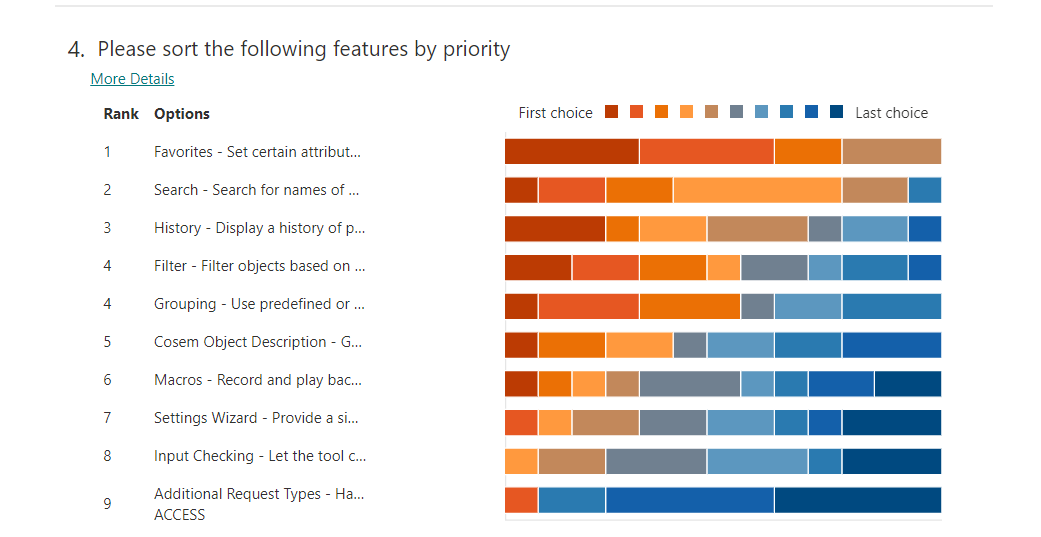
\includegraphics[width=1.0\textwidth]{gfx/S1_Survey_Prio.png}
   \caption{
       Resultat der Umfrage: Sortiere diese Features nach Priorität
   }
   \label{fig:FeaturesPrio}
\end{figure}

Die Nutzer wurden ebenfalls dazu befragt, auf welchen Plattformen sie die neue Anwendung gerne einsetzten würden.
Im nächsten Abschnitt werden die Antworten (Abbildung \ref{fig:SurveryPlatforms}) auf diese Frage sowie viele weitere Aspekte für die Evaluation des Technologiestacks verwendet.

\begin{figure}[H]
   \centering
   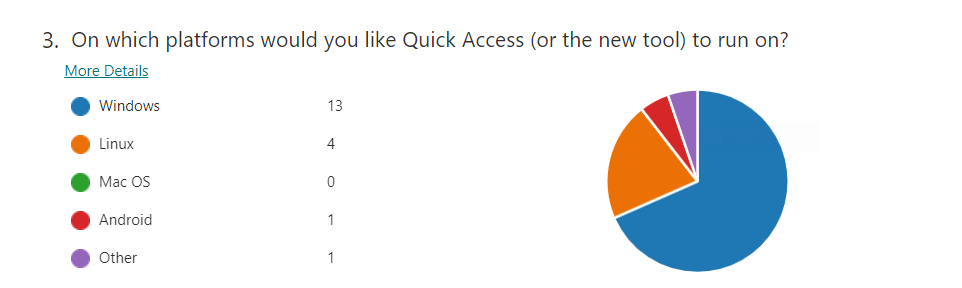
\includegraphics[width=1.0\textwidth]{gfx/S0_Survey_Platform.png}
   \caption{
       Resultat der Umfrage: Gewünschte Plattformen
   }
   \label{fig:SurveryPlatforms}
\end{figure}

\subsection{Evaluation des Technologiestacks}

\subsection{Erstellung des Backlogs}
Wie in Abschnitt \ref{methoden:ADO} erklärt, wurde \ac{ADO} für die Verwaltung des Backlogs verwendet.
Dazu musste als erstes eine neues \ac{ADO} Projekt erstellt und die Sprints eingetragen werden.
Nun konnten User Stories formuliert und auf die sechs geplanten Sprints verteilt werden.


% TODO no chli meh schribe?

Welche Stories im ersten Sprint bearbeitet wurden und wie dies genau ablief ist im folgenden Kapitel zu lesen.
